\documentclass[conference]{IEEEtran}
\IEEEoverridecommandlockouts
\usepackage{cite}
\usepackage{amsmath,amssymb,amsfonts}
\usepackage{graphicx}
\usepackage{textcomp}
\usepackage{xcolor}
\usepackage{booktabs}
\usepackage{multirow}
\usepackage{placeins}
\usepackage{enumitem}
\usepackage{hyperref}
\hypersetup{hidelinks}
\usepackage{tikz}
\usetikzlibrary{arrows.meta,positioning,calc}

\newcommand{\wasm}{\textnormal{\textsc{wasm}}}
\newcommand{\ms}{\,ms}

\definecolor{hwblue}{RGB}{180,205,240}
\definecolor{osbrown}{RGB}{255,200,100}
\definecolor{wgreen}{RGB}{144,220,144}
\definecolor{cpurple}{RGB}{210,185,235}
\definecolor{cblue}{RGB}{150,195,235}
\definecolor{yorange}{RGB}{220,155,130}
\definecolor{gpink}{RGB}{255,200,200}

\begin{document}

\title{Web-Based Edge Computing for Optical Mark Recognition:\protect\\
A Cross-Platform Performance Benchmark}

\author{%
\IEEEauthorblockA{%
Faculty of Information Systems\\
University of Information Technology, VNU-HCM\\
Ho Chi Minh City, Vietnam}
\vspace{0.35em}
\IEEEauthorblockN{%
\begin{tabular}{@{}c@{\hspace{2.6em}}c@{\hspace{2.6em}}c@{}}
Huy Kien Phan & Minh Chau Truong & Thanh Binh Nguyen
\end{tabular}}
\IEEEauthorblockA{%
\begin{tabular}{@{}c@{\hspace{2.6em}}c@{\hspace{2.6em}}c@{}}
\texttt{huykien283@gmail.com} & \texttt{chautm@uit.edu.vn} & \texttt{binhnt@uit.edu.vn}
\end{tabular}}
}

\maketitle

\begin{abstract}
Browser-based Optical Mark Recognition (OMR) can keep student answer
sheets on-device and avoid application installation, but its practical
performance depends on more than neural-network inference. This paper
benchmarks a complete Web Edge OMR pipeline that combines WebAssembly
(\wasm{}) computer vision with WebGPU YOLO inference, and compares it
with a Native Android baseline on a reviewed 179-sheet set across six
Web hosts and one mobile device. The Web CV path reaches 99.00\%
question accuracy, and the YOLO handoff study shows that detector
localization must be validated against the downstream fixed-template
recognizer rather than treated as an automatic accuracy gain. The main
result is stage attribution: WebGPU makes YOLO inference secondary,
while deterministic CV running through \wasm{} dominates end-to-end
latency. On the current $N{=}179$ set, the same-boundary CV
\texttt{cpp\_ms} gap between Mobile Web and Native is $7.0\times$, and on
the same processing boundary Mobile Web YOLO \texttt{cpp\_ms} remains
$2.83\times$ slower than Native NNAPI. These
results show that competitive Web Edge OMR depends primarily on
reducing \wasm{} CV overhead, not further accelerating YOLO inference.
\end{abstract}

\begin{IEEEkeywords}
Optical mark recognition, edge computing, web browser, YOLO,
WebAssembly, WebGPU, cross-platform benchmark
\end{IEEEkeywords}

\section{Introduction}

Automated grading of multiple-choice answer sheets is widely used in
educational institutions, where large volumes of sheets must be
processed accurately within a short time. Existing deployments follow
two established patterns. Server-based services transmit scanned or
photographed sheets to remote infrastructure, introducing network
dependency and exposing student data to external
systems~\cite{patel2015,okorie2022}. Native mobile applications avoid
data transmission but require platform-specific packaging, app-store
distribution, and per-platform maintenance overhead.

Recent advances in \wasm{} and WebGPU enable computer-vision and
deep-learning workloads to execute directly inside modern web browsers
without plugins or installation. This creates a third deployment model:
a fully client-side pipeline in which answer-sheet images are processed
entirely within the browser and never transmitted to any server. The
same URL-deployed code bundle runs across desktop and mobile browsers,
removing both the data-exposure risk of server-side grading and the
installation friction of native applications.

Realizing this model requires two heterogeneous execution paths within
the browser sandbox. Classical image-processing stages---perspective
rectification, adaptive thresholding, and fixed-grid bubble
reading---are compiled from C\texttt{++}/OpenCV to \wasm{} and execute on
the CPU. Neural-network inference for sheet-region localization uses ONNX
Runtime Web with a WebGPU backend. These two paths operate under
different browser APIs and on different hardware, so their relative cost
determines whether the combined pipeline is competitive with native
execution.

This paper studies whether WebGPU inference is enough to make a Web
Edge OMR pipeline competitive with Native Android. The answer is no
under the measured workload: WebGPU reduces YOLO latency, but the
deterministic CV/\wasm{} stage dominates end-to-end behavior. Native
Android remains the lower-latency deployment; Web Edge is the
privacy-preserving and URL-deployed trade-off whose competitiveness
depends on bounding the \wasm{} CV stage.

The paper makes three contributions:
\begin{enumerate}[leftmargin=*, itemsep=1pt, topsep=2pt]
  \item A reviewed cross-platform OMR benchmark on a 179-sheet set with
  supervised accuracy, latency, and resource measurements across six Web
  Edge hosts and one Native Android baseline.
  \item A stage-attribution result showing that \wasm{} OMR, not YOLO
  inference, is the dominant bottleneck: the same-round CV
  \texttt{cpp\_ms} gap between Mobile Web and Native is $7.0\times$, and
  Mobile Web YOLO \texttt{cpp\_ms} is $2.83\times$ the Native NNAPI
  boundary.
  \item A YOLO handoff analysis: raw handoff preserves the 99.00\% CV
  recognition score, but detector hard masks drop to 63.70\% and
  74.40\%, so bbox-guided cropping must be validated separately.
\end{enumerate}

\section{Related Work}

\paragraph{Classical OMR}
Traditional OMR pipelines rely on handcrafted image-processing
techniques such as thresholding, edge detection, and morphological
operations for bubble localization and recognition~\cite{patel2015,okorie2022}.
Although computationally efficient, these methods remain sensitive to
illumination variation and geometric distortion in mobile capture
scenarios~\cite{afifi2019}.

\paragraph{Deep learning for OMR}
Recent studies adopt YOLO-based detectors~\cite{redmon2016} to improve
robustness under challenging imaging conditions. Ali et
al.~\cite{ali2025} show that YOLO achieves higher detection accuracy and
better generalization than threshold-based approaches, while
YOLOv8n~\cite{jocher2023} provides a lightweight architecture suitable
for edge deployment. Tabassum and Rahman~\cite{tabassum2024} deploy
YOLOv8 for mobile OMR but report neither stage-level latency
decomposition nor a controlled cross-platform comparison, leaving
unclear how inference cost relates to the surrounding CV pipeline on
constrained devices.

\paragraph{Browser-based edge computing}
\wasm{} and WebGPU enable privacy-preserving client-side execution in
modern browsers, with neural inference exposed through ONNX Runtime
Web~\cite{microsoft2021}. Jangda et al.~\cite{jangda2019} report that
\wasm{} is on average 45\% slower than native execution on
compute-intensive benchmarks, indicating potential overhead for
C\texttt{++} image-processing workloads compiled to \wasm{}. Wang et
al.~\cite{wang2024} find browser DL inference to be $16.9\times$ slower
than native on CPU and $4.9\times$ on GPU, with WebGPU providing the
best browser-side performance among the evaluated back-ends.
Nevertheless, these evaluations focus on isolated workloads rather than
complete computer-vision pipelines. The emerging W3C WebNN
API~\cite{webnn2024} provides a higher-level hardware-abstraction layer
for neural-network acceleration in the browser, but the current draft
remains a work in progress. Consequently, the interaction between
\wasm{}-based image processing and WebGPU inference in real applications
remains insufficiently understood.

\paragraph{Research gap}
Existing work studies either OMR accuracy or browser inference
performance in isolation. To our knowledge, no prior study has evaluated
a fully client-side browser OMR pipeline in which both computer vision
and neural inference are executed locally without transmitting
answer-sheet data to external servers. Furthermore, it remains unclear
whether end-to-end latency is dominated by neural inference or by
\wasm{}-executed computer vision stages. This paper addresses these gaps
through controlled per-stage profiling of a YOLOv8n-based browser OMR
system across multiple execution back-ends and deployment configurations.

\section{System Architecture and Methods}

\begin{figure}[t]
  \centering
  \resizebox{\columnwidth}{!}{%
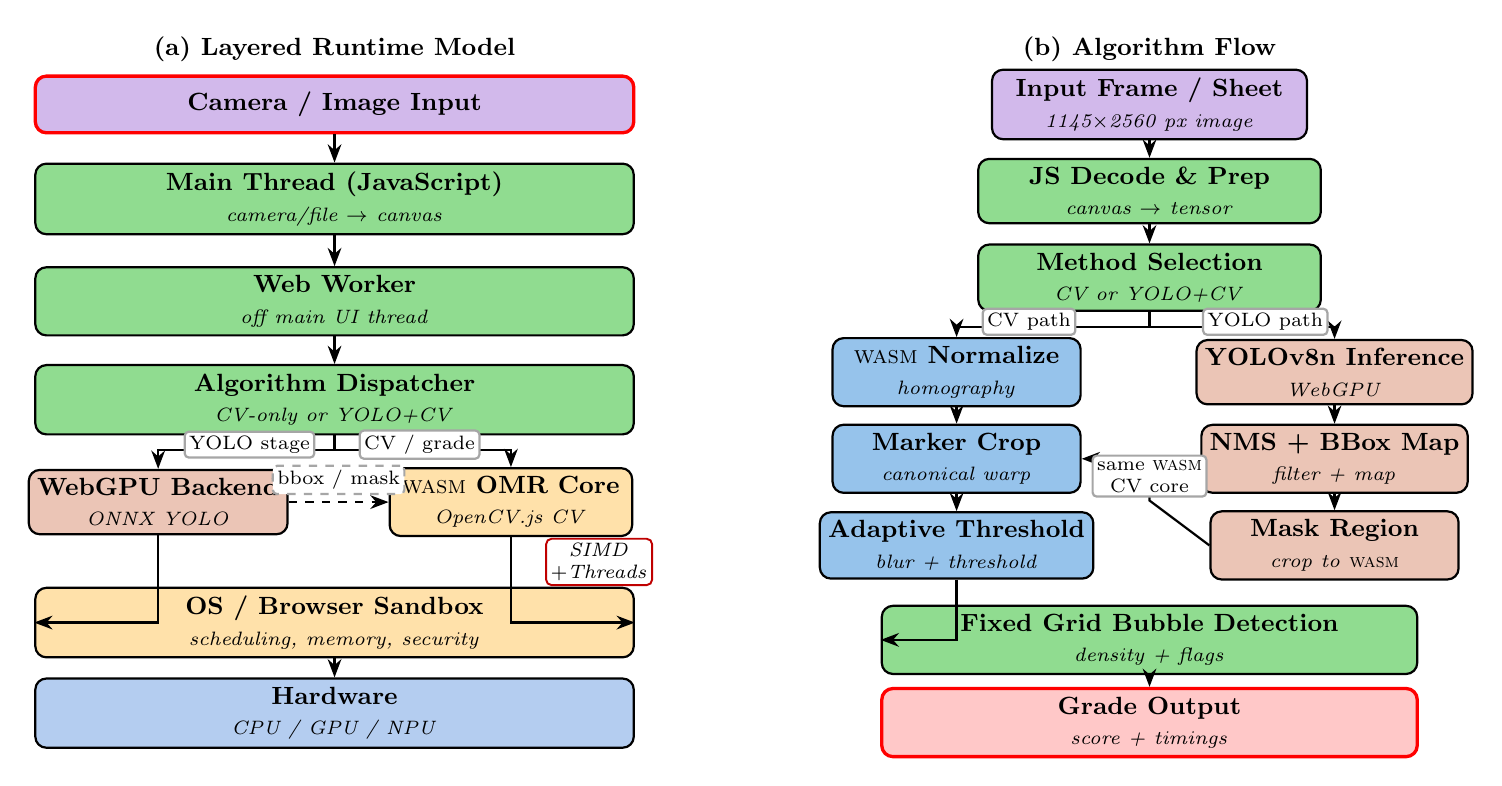
\begin{tikzpicture}[
  font=\small,
  >=Stealth,
  thick,
  every node/.style={align=center},
  base/.style    = {draw, rounded corners=4pt, text centered, inner sep=3pt, text=black},
  wide/.style    = {base, minimum width=7.6cm, minimum height=0.72cm},
  mid/.style     = {base, minimum width=3.08cm, minimum height=0.78cm},
  small/.style   = {base, minimum width=3.15cm, minimum height=0.70cm},
  camnd/.style   = {wide, fill=cpurple, draw=red, line width=1.2pt},
  wknd/.style    = {wide, fill=wgreen},
  dispnd/.style  = {wide, fill=wgreen, minimum height=0.88cm},
  osnd/.style    = {wide, fill=osbrown!55},
  hwnd/.style    = {wide, fill=hwblue},
  wgpund/.style  = {mid, fill=yorange!58},
  wasmnd/.style  = {mid, fill=osbrown!55},
  cfrnd/.style   = {base, fill=cpurple, minimum width=4.00cm, minimum height=0.72cm},
  jsnd/.style    = {base, fill=wgreen, minimum width=4.35cm, minimum height=0.72cm},
  cvbx/.style    = {small, fill=cblue},
  ylbx/.style    = {small, fill=yorange!58},
  mrgnd/.style   = {base, fill=wgreen, minimum width=6.8cm, minimum height=0.78cm},
  outnd/.style   = {base, fill=gpink, draw=red, line width=1.2pt,
                    minimum width=6.8cm, minimum height=0.68cm},
  simdlbl/.style = {draw=red!75!black, line width=0.7pt, fill=white,
                    rounded corners=2pt, inner sep=1.6pt, font=\scriptsize},
  lab/.style     = {draw=black!35, fill=white, rounded corners=1.5pt,
                    inner sep=1.6pt, font=\scriptsize}
]
\node[hwnd] (hw) at (0.00, 0.02)
  {\textbf{Hardware} \\ \textit{\scriptsize CPU / GPU / NPU}};
\node[osnd] (os) at (0.00, 1.17)
  {\textbf{OS / Browser Sandbox} \\ \textit{\scriptsize scheduling, memory, security}};
\node[wasmnd] (wasm) at ( 2.24, 2.70)
  {\textbf{\wasm{} OMR Core} \\ \textit{\scriptsize OpenCV.js CV}};
\node[wgpund] (wgpu) at (-2.24, 2.70)
  {\textbf{WebGPU Backend} \\ \textit{\scriptsize ONNX YOLO}};
\node[dispnd] (disp) at (0.00, 4.00)
  {\textbf{Algorithm Dispatcher} \\ \textit{\scriptsize CV-only or YOLO+CV}};
\node[wknd] (wk) at (0.00, 5.25)
  {\textbf{Web Worker} \\ \textit{\scriptsize off main UI thread}};
\node[wknd] (mt) at (0.00, 6.55)
  {\textbf{Main Thread (JavaScript)} \\
   \textit{\scriptsize camera/file $\to$ canvas}};
\node[camnd] (cam) at (0.00, 7.75)
  {\textbf{Camera / Image Input}};

\draw[->] (cam) -- (mt);
\draw[->] (mt) -- (wk);
\draw[->] (wk) -- (disp);
\coordinate (dispatchSplit) at (0.00, 3.36);
\draw[->] (disp.south) -- (dispatchSplit) -| (wgpu.north);
\draw[->] (disp.south) -- (dispatchSplit) -| (wasm.north);
\node[lab] at (-1.08, 3.43) {YOLO stage};
\node[lab] at ( 1.08, 3.43) {CV / grade};
\draw[->, dashed] (wgpu.east) -- node[lab, midway, above=2.5pt] {bbox / mask} (wasm.west);
\draw[->] (wgpu.south) -- ++(0,-0.58) |- (os.west);
\draw[->] (wasm.south) -- ++(0,-0.58) |- (os.east);
\draw[->] (os) -- (hw);
\node[simdlbl] at (3.36, 1.94) {\textit{SIMD} \\ +\textit{Threads}};
\node[font=\small\bfseries] at (0.00, 8.45) {(a) Layered Runtime Model};

\node[cfrnd] (cfr) at (10.35, 7.75)
  {\textbf{Input Frame / Sheet} \\ \textit{\scriptsize 1145$\times$2560 px image}};
\node[jsnd] (decode) at (10.35, 6.65)
  {\textbf{JS Decode \& Prep} \\ \textit{\scriptsize canvas $\to$ tensor}};
\node[jsnd] (select) at (10.35, 5.55)
  {\textbf{Method Selection} \\ \textit{\scriptsize CV or YOLO+CV}};
\node[cvbx] (cvnorm) at (7.90, 4.35)
  {\textbf{\wasm{} Normalize} \\ \textit{\scriptsize homography}};
\node[cvbx] (stage2) at (7.90, 3.25)
  {\textbf{Marker Crop} \\ \textit{\scriptsize canonical warp}};
\node[cvbx] (thr) at (7.90, 2.15)
  {\textbf{Adaptive Threshold} \\ \textit{\scriptsize blur + threshold}};
\node[ylbx] (yolo) at (12.70, 4.35)
  {\textbf{YOLOv8n Inference} \\ \textit{\scriptsize WebGPU}};
\node[ylbx] (nms) at (12.70, 3.25)
  {\textbf{NMS + BBox Map} \\ \textit{\scriptsize filter + map}};
\node[ylbx] (mask) at (12.70, 2.15)
  {\textbf{Mask Region} \\ \textit{\scriptsize crop to \wasm{}}};
\node[mrgnd] (grid) at (10.35, 0.95)
  {\textbf{Fixed Grid Bubble Detection} \\ \textit{\scriptsize density + flags}};
\node[outnd] (grade) at (10.35, -0.10)
  {\textbf{Grade Output} \\ \textit{\scriptsize score + timings}};

\draw[->] (cfr) -- (decode);
\draw[->] (decode) -- (select);
\coordinate (methodSplit) at (10.35, 4.92);
\draw[->] (select.south) -- (methodSplit) -| (cvnorm.north);
\draw[->] (select.south) -- (methodSplit) -| (yolo.north);
\node[lab] at (8.82, 4.99) {CV path};
\node[lab] at (11.82, 4.99) {YOLO path};
\draw[->] (cvnorm) -- (stage2);
\draw[->] (stage2) -- (thr);
\draw[->] (yolo) -- (nms);
\draw[->] (nms) -- (mask);
\coordinate (coreLink) at (10.35, 2.72);
\draw[->] (mask.west) -- (coreLink) |- (stage2.east);
\node[lab, font=\scriptsize] at (10.35, 3.03) {same \wasm{}\\CV core};
\draw[->] (thr.south) |- (grid.west);
\draw[->] (grid) -- (grade);
\node[font=\small\bfseries] at (10.35, 8.45) {(b) Algorithm Flow};
\end{tikzpicture}%
  }
  \caption{Web-Based Edge OMR architecture. The main JavaScript thread
  dispatches camera or file input to a Web Worker. WebGPU accelerates
  only YOLO localization; normalization, thresholding, bubble reading,
  and grading remain in the \wasm{} C\texttt{++}/OpenCV core.}
  \label{fig:arch}
\end{figure}

\subsection{Cross-Platform System Architecture}
The system adopts a layered runtime architecture for on-device OMR,
illustrated in Fig.~\ref{fig:arch}(a). Image data acquired from a camera
stream or uploaded file is first received by the JavaScript main thread,
which handles user interaction and data acquisition. The image is then
transferred to a dedicated Web Worker so that computation does not block
UI responsiveness. Within the worker, an Algorithm Dispatcher selects
either a conventional CV-only pipeline or a hybrid YOLO$+$CV pipeline. In
the hybrid configuration, object localization is performed by an
ONNX-based YOLO model on a WebGPU backend, while image processing and
grading run in a \wasm{} OMR core built on OpenCV.js. Localization
outputs (bounding boxes or masks) are forwarded to the \wasm{} module, so
both pipelines share the same grading workflow. The WebGPU and \wasm{}
backends operate within the OS/Browser sandbox, which manages scheduling,
memory, and security while mapping work onto the available CPU, GPU, and
NPU. This layered design separates application control, algorithm
execution, and hardware abstraction, providing a unified implementation
across heterogeneous platforms.

\subsection{Pipeline}

Fig.~\ref{fig:arch} separates the runtime stack from the algorithmic
flow. The worker executes either a CV-only path or a YOLO$+$CV path.
The CV path performs grayscale/blur preprocessing, marker or paper
boundary detection, homography into a canonical $1700\times2400$
template, adaptive thresholding, and fixed-grid bubble-density reading.
The YOLO path fine-tunes YOLOv8n for four localization classes
(\texttt{marker\_corners}, \texttt{id\_keycode},
\texttt{questions\_1\_20}, \texttt{questions\_21\_60}); inference uses a
$640\times640$ letterboxed tensor, confidence filtering, and NMS before
passing a retained region to the same CV recognizer.

The CV recognizer is intentionally deterministic. Marker candidates are
derived from thresholded connected components and geometric filters; if
the marker route is unreliable, a paper-boundary fallback estimates the
sheet corners. The selected quadrilateral defines a homography into the
template coordinate system, after which bubble centers are fixed by the
known grid. Each option is scored by foreground density inside a circular
sampling window and then normalized at the row level. This design makes
the algorithm fast and reproducible, but also means that small geometric
changes introduced before the homography stage can propagate into the
entire answer grid.

YOLO is therefore used as a localization stage rather than as a direct
answer classifier. It can identify regions such as the marker corners
and question blocks, but the answer string remains the output of the CV
recognizer. This separation is useful for benchmarking because it lets
the paper distinguish three cases: CV-only recognition, YOLO inference
with raw handoff, and YOLO hard masks that alter the image entering the
recognizer. The accuracy ablation in Section~\ref{sec:results-recognition}
follows directly from these handoff modes.

This split is imposed by the Web platform. OpenCV.js exposes the CV
pipeline through \wasm{}, while ONNX Runtime Web can execute YOLO via
WebGPU. Thus WebGPU accelerates learned localization but not
homography, thresholding, or grading. Native Android uses OpenCV through
Kotlin/JNI and ONNX Runtime Android with CPU 1T, CPU 4T, and NNAPI
providers. Native Android is used only as a latency/resource baseline:
the current Android benchmark does not export per-question Native YOLO
labels aligned to the reviewed ground truth, so no Native accuracy
claim is made.

The benchmark treats runtime differences as part of the deployment
environment. OpenCV.js and OpenCV Android share source-level algorithmic
stages but not binary implementation details: OpenCV version, memory
layout, SIMD scheduling, floating-point ordering, and image-buffer
marshalling can differ. The same exported ONNX model is used for Web and
Native inference to avoid framework-conversion variance, but the
execution providers are intentionally platform-native: WebGPU in the
browser and CPU/NNAPI on Android.

\subsection{Platform-Specific Optimization and Deployment}
The two deployment targets offer complementary trade-offs. The Web Edge
implementation employs OpenCV.js and WebGPU, enabling cross-platform
execution and browser deployment without installation; however, browser
sandboxing introduces additional overhead and limits direct access to
hardware accelerators. The Native Android implementation instead uses the
OpenCV Android SDK and ONNX Runtime Android, allowing direct hardware
acceleration through frameworks such as NNAPI and thus lower inference
latency, at the cost of increased packaging and per-platform maintenance
complexity. Unlike conventional cloud-based mobile OMR, both deployments
perform all processing locally on the device, eliminating network
latency, enabling offline operation, and avoiding data transmission to
external servers; compared with server-side OMR, this edge-computing
approach also removes the need for dedicated server infrastructure and
reduces operational cost.

\section{Experimental Setup}

The $N{=}179$ system set contains five sub-datasets
(\texttt{dataset\_1}=48, \texttt{dataset\_2}=47,
\texttt{dataset\_3}=35, \texttt{dataset\_4}=45,
\texttt{dataset\_5}=4) captured at $1{,}145\times2{,}560$\,px on a
Redmi Note~13 Pro+. A human-reviewed CSV under
\texttt{runs/accuracy\_eval/} marks invalid trailing questions as
\texttt{NA}, yielding 9,488 valid question labels and 47,440 binary
A/B/C/D/E bubble decisions. YOLO training uses 56 manually annotated
sheets (45 train, 11 validation) with the default Ultralytics YOLOv8n
recipe and a single exported ONNX model shared by Web and Native.

Six Web hosts replay the same $N{=}179$ images: a desktop reference
(i5-14600K/RTX 4070 Ti SUPER), ASUS Vivobook (i5-13500H), Acer Nitro~5
(i5-10300H), MacBook Air M1, iPhone~16 Safari/WebKit, and Redmi
Note~13 Pro+ Chrome/Blink. The Native Android baseline runs on the same
Redmi device. Web latency rows report worker-side \texttt{cpp\_ms};
Native rows report file-based \texttt{e2e\_ms}. Same-boundary
statistical tests use \texttt{cpp\_ms} on both Web and Native.
Resources use the instrument available on each host: \texttt{psutil}
for Windows Chrome, an in-page timer-lag proxy for browser hosts where
process sampling is unavailable, and an Android in-app sampler for
Native.

\begin{table}[t]
\caption{Benchmark artifacts and metric boundaries.}
\label{tab:metrics}
\centering
\setlength{\tabcolsep}{3pt}
\resizebox{\columnwidth}{!}{%
\begin{tabular}{lll}
\toprule
\textbf{Claim} & \textbf{Primary artifact} & \textbf{Boundary} \\
\midrule
Recognition & \texttt{runs/accuracy\_eval/} & valid questions only \\
Web latency & \texttt{runs/batch\_results/} & worker \texttt{cpp\_ms} \\
Web YOLO handoff & Redmi raw-handoff + detection summary & worker total timer \\
Native latency & Native JSON files & file-based \texttt{e2e\_ms} \\
Stage attribution & stage profiles + Native logs & stage timers \\
Resources & \texttt{runs/resources/} CSVs & instrument-specific \\
\bottomrule
\end{tabular}}
\vspace{2pt}
\parbox{\columnwidth}{\footnotesize
The table separates same-boundary comparisons from deployment-boundary
comparisons. Web browser wall-time is not exported by the current batch
logs.}
\end{table}

Table~\ref{tab:metrics} summarizes the evidence boundary for each
claim. Accuracy is a direct supervised comparison against the
human-reviewed CSV. Web \texttt{cpp\_ms} starts after image data reaches
the worker and excludes main-thread decode and UI work; Native
\texttt{e2e\_ms} includes file decode, processing, and debug write. The
paper therefore avoids presenting the Web-vs-Native rows as a strict
full-E2E race. When a same-boundary ratio is needed, both sides use
\texttt{cpp\_ms}; when deployment latency is discussed, the boundary is
stated in the caption or text.

\section{Results and Discussion}

\subsection{Recognition Accuracy}
\label{sec:results-recognition}

Table~\ref{tab:accuracy} reports supervised exact-match recognition on
the reviewed $N{=}179$ artifact. Traditional CV correctly recognizes
9,393 of 9,488 valid questions (99.00\%) and exactly matches all valid
questions on 137 of 179 sheets. The YOLO raw-handoff row is identical
by construction: YOLO is executed, but the downstream C\texttt{++}
recognizer receives the same unmasked image as CV-only. In contrast,
the configurations that actually consume YOLO hard masks drop to
63.70\% (12\% bbox expansion) and 74.40\% (20\%), showing that
detector-assisted cropping can destabilize the fixed-template grid.
At the bubble level, the reviewed artifact gives Precision 0.992,
Recall 0.994, and F1 0.993 for CV and raw-handoff YOLO.

This negative result is important for interpreting YOLO's role. The
raw-handoff row should not be read as a detector-driven accuracy gain:
it executes the detector but intentionally leaves the recognizer input
unchanged. It is included to keep the latency pipeline complete while
avoiding a recognition algorithm change. A separate handoff audit under
\texttt{runs/accuracy\_eval/yolo\_detection\_n179/} shows that this
raw path completed on all 179 sheets with zero fallback, while the
detector flag itself is true for 154 sheets. The hard-mask rows are the
actual detector-consuming variants, and their large drop shows that a
detector run is not sufficient for fixed-template OMR.
Small changes to the crop boundary alter marker refinement and the
downstream bubble grid, especially on lightly filled or marginally
photographed sheets. For this reason, bbox-guided cropping is treated
as a separate recognition algorithm rather than a harmless preprocessor.

\begin{table}[t]
\caption{Supervised question-level recognition accuracy on the reviewed
$N{=}179$ set.}
\label{tab:accuracy}
\centering
\setlength{\tabcolsep}{3pt}
\resizebox{\columnwidth}{!}{%
\begin{tabular}{lcccccc}
\toprule
\textbf{Method} & \textbf{Q Acc.} & \textbf{Correct/GT Qs.}
& \textbf{Sheet Exact} & \textbf{GT Blank}
& \textbf{Pred Blank} & \textbf{Pred Multi} \\
\midrule
Traditional CV              & \textbf{99.00\%} & \textbf{9{,}393}/9{,}488 & \textbf{137}/179 & 44 & 42  & 18 \\
YOLO + CV, raw handoff      & 99.00\%          & 9{,}393/9{,}488          & 137/179          & 44 & 42  & 18 \\
YOLO + CV, hard mask (12\%) & 63.70\%          & 6{,}044/9{,}488          & 84/179           & 44 & 987 & 231 \\
YOLO + CV, hard mask (20\%) & 74.40\%          & 7{,}059/9{,}488          & 101/179          & 44 & 614 & 199 \\
\bottomrule
\end{tabular}}
\vspace{2pt}
\parbox{\columnwidth}{\footnotesize
Artifacts are under \texttt{runs/accuracy\_eval/} and the Redmi YOLO
raw-handoff batch JSON. Bubble-level CV/raw-handoff metrics are
P=0.992, R=0.994, F1=0.993 over 47,440 binary decisions.}
\end{table}

\subsection{Cross-Platform Latency}
\label{sec:latency}

Table~\ref{tab:latency} and Fig.~\ref{fig:latency} report the
deployment benchmark. WebGPU makes ML inference secondary: warm YOLO
inference falls from $1{,}170$\,ms to $142$\,ms on the desktop reference
profile, but Mobile Web YOLO raw-handoff still reports $669\pm30$\,ms
\texttt{cpp\_ms} and $998\pm75$\,ms worker-total time. Native Android
on the same Redmi device reaches $264\pm17$\,ms file-based E2E with
NNAPI.

\begin{figure}[!b]
  \centering
  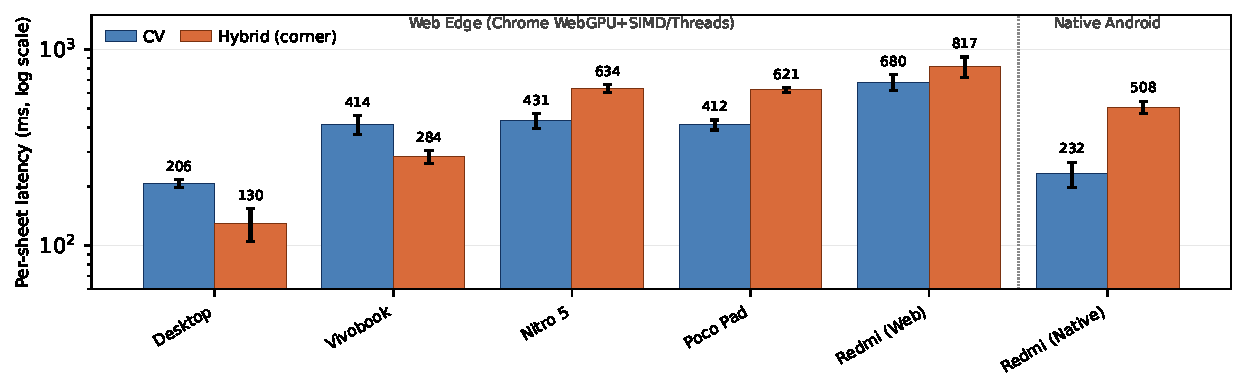
\includegraphics[width=\columnwidth]{figures/fig1_latency.pdf}
  \caption{Per-sheet latency by platform and configuration
  ($N{=}179$, log scale). Web bars are \texttt{cpp\_ms}; Native bars are
  file-based \texttt{e2e\_ms}.}
  \label{fig:latency}
\end{figure}

The reason is the deterministic CV stage. In the Mobile Web
SIMD$+$Threads stage-decomposition profile ($N{=}43$, Chrome v120,
original measurement round), \wasm{} OMR takes $1{,}124$\,ms, whereas
native C\texttt{++}/OpenCV OMR measured on the current artifact
takes $\approx 88$\,ms. The $12.8\times$ ratio is therefore
an upper bound; a same-round, same-boundary comparison on the current
$N{=}179$ set (Mobile Web CV \texttt{cpp\_ms} $615\pm23$ versus Native CV
\texttt{cpp\_ms} $88\pm9$) still gives a $7.0\times$ gap. On the same
processing boundary, Mobile Web
YOLO \texttt{cpp\_ms} ($669\pm30$\,ms) versus the Native NNAPI
\texttt{cpp\_ms} portion ($236\pm15$\,ms) of the $264$\,ms E2E row in
Table~\ref{tab:latency} gives $2.83\times$ after excluding JPEG decode
and debug write. Same-boundary \texttt{cpp\_ms} Welch tests are
significant for every Web-vs-Native provider pair.

SIMD and threading reduce, but do not remove, the bottleneck. The
OpenCV.js SIMD$+$Threads build reduces OMR by $18.7\times$ on the
desktop reference host and by $12.7\times$ on the Redmi stage profile.
Yet if the Mobile Web YOLO profile simply substituted native OMR speed
($\approx 88$\,ms) for \wasm{} OMR ($1{,}124$\,ms), Web YOLO E2E would be
$\approx 387$\,ms, only $1.46\times$ above Native NNAPI. This
counterfactual shows that CV/\wasm{} execution, not YOLO, drives the
remaining pipeline-level gap.

Table~\ref{tab:stage-mini} makes the stage attribution explicit. The
desktop rows show that SIMD$+$Threads can move OpenCV.js from an
unusable warm profile toward sub-second processing. The Redmi rows show
why that improvement still does not close the deployment gap: WebGPU
YOLO inference is within a factor of two of NNAPI ORT time
($299$ vs.\ $158$\,ms), but the CV stage remains more than an order of
magnitude slower in the older Mobile Web profile. Thus replacing the
detector backend alone can only shift a secondary term once WebGPU is
enabled; the first-order term is the OMR implementation boundary.

\begin{table}[t]
\caption{Stage-attribution profiles used to interpret the deployment
latency. Stage rows are context-specific profiles, not a pooled
benchmark; they identify which stage dominates after WebGPU is enabled.}
\label{tab:stage-mini}
\centering
\setlength{\tabcolsep}{2.5pt}
\resizebox{\columnwidth}{!}{%
\begin{tabular}{llccc}
\toprule
\textbf{Host/context} & \textbf{Runtime} & \textbf{YOLO/ORT} & \textbf{OMR} & \textbf{Total} \\
\midrule
Desktop warm frame & \wasm{} only & $1{,}170$ & $8{,}175$ & $9{,}360$ \\
Desktop $N{=}54$ & WebGPU+SIMD+Threads & $81\pm12$ & $438\pm11$ & $643\pm23$ \\
Redmi $N{=}43$ & WebGPU+SIMD+Threads & $299\pm50$ & $\approx 1{,}124$ & $1{,}423\pm163$ \\
Redmi $N{=}179$ & Native NNAPI & $158\pm11$ & $106\pm11$ & $264\pm17$ \\
\bottomrule
\end{tabular}}
\vspace{2pt}
\parbox{\columnwidth}{\footnotesize
Times are milliseconds. Desktop and Redmi Web rows are stage profiles;
the Native row is the current file-based headless run. Native total is
E2E and includes JPEG decode plus debug write; Native OMR is
\texttt{cpp\_ms}. Stage timers do not necessarily sum to Total because
browser scheduling, GPU dispatch, and post-processing are outside the
YOLO/ORT and OMR timer boundaries.}
\end{table}

\begin{table}[t]
\caption{Per-sheet latency across seven host configurations
($N{=}179$). Web rows report \texttt{cpp\_ms}; Native rows report
file-based \texttt{e2e\_ms}.}
\label{tab:latency}
\centering
\resizebox{\columnwidth}{!}{%
\begin{tabular}{llcc}
\toprule
\textbf{Platform} & \textbf{Stack} & \textbf{CV (ms)} & \textbf{YOLO (ms)} \\
\midrule
\multicolumn{4}{l}{\textit{Web Edge --- WebGPU+SIMD+Threads unless noted}} \\
Desktop reference & Win/Blink & $248\pm15$ & $246\pm18$ \\
Laptop (Vivobook) & Win/Blink & $585\pm124$ & $628\pm161$ \\
Laptop (Nitro~5)  & Win/Blink & $427\pm35$ & $423\pm40$ \\
Mac (M1)          & macOS/Blink & $240\pm16$ & $240\pm22$ \\
Mobile (Redmi)    & Android/Blink & $615\pm23$ & $669\pm30$ \\
iPhone~16         & iOS/WebKit/SIMD only & $\mathbf{160\pm14}$ & $\mathbf{165\pm18}$ \\
\midrule
\multicolumn{4}{l}{\textit{Native Android on Redmi}} \\
\multirow{3}{*}{Native Android} & CPU 1T & $118\pm14$ & $509\pm38$ \\
                                & CPU 4T & n/a & $375\pm29$ \\
                                & NNAPI  & n/a & $\mathbf{264\pm17}$ \\
\bottomrule
\end{tabular}}
\vspace{2pt}
\parbox{\columnwidth}{\footnotesize
The Redmi Web YOLO row is the raw-handoff run; its worker-total timer
including inference is $998\pm75$\,ms. Web browser wall-time is not
exported in the current batch JSON. Native E2E includes JPEG decode,
processing, and debug write. The Vivobook row is a five-run
High-Performance mean$\pm$std (Sec.~\ref{sec:threats}); other Web rows
are single runs.}
\end{table}

\FloatBarrier

\subsection{System Resource Usage}
\label{sec:resources}

Resources remain bounded over the continuous run
(Table~\ref{tab:resources}, Fig.~\ref{fig:cross_platform}). CPU units
are instrument-specific:
Windows rows use renderer-process CPU\%, Mac/iOS/Android Web rows use
the in-page event-loop proxy, and Native rows use an Android sampler out
of $800\%$ on the 8-core SoC. The highest observed Web peak is
$\approx 1.3$\,GB on the desktop reference/Vivobook-class Windows
Chrome hosts; Native peaks at 702\,MB for CV and 645\,MB for YOLO.
These numbers support feasibility on mid-range devices, but they should
not be interpreted as direct CPU-efficiency ratios across instruments.

\begin{table}[!t]
\caption{Resource summary over the $N{=}179$ continuous run. CPU cells
are avg/peak in the instrument's native unit; RAM cells are CV/YOLO peak
MB.}
\label{tab:resources}
\centering
\scriptsize
\setlength{\tabcolsep}{2.5pt}
\resizebox{\columnwidth}{!}{%
\begin{tabular}{lcccl}
\toprule
\textbf{Host} & \textbf{CV CPU} & \textbf{YOLO CPU}
& \textbf{RAM} & \textbf{Instr.} \\
\midrule
Desktop & $60.5/168.7\%$ & $55.7/76.5\%$ & $1{,}310/984$ & psutil \\
Vivobook & $96.8/225.2\%$ & $85.3/156.9\%$ & $1{,}137/1{,}001$ & psutil \\
Nitro~5 & $74.7/204.6\%$ & $74.1/98.4\%$ & $1{,}145/1{,}071$ & psutil \\
M1 Mac & $0.59/0.89$ & $0.67/0.85$ & $1{,}073/248$ & proxy \\
iPhone~16 & $0.04/0.84$ & $0.21/0.83$ & $147/147$ & proxy \\
Redmi Web & $0.65/1.40$ & $0.54/1.74$ & $147/147$ & proxy \\
Native & $360/462\%$ & $237/525\%$ & $702/645$ & sampler \\
\bottomrule
\end{tabular}}
\vspace{1pt}
\parbox{\columnwidth}{\footnotesize
RAM values are MB peak RSS or browser-exposed heap/\wasm{} memory. Safari
does not expose full JavaScript heap telemetry; Mac/iPhone memory is
therefore a lower-bound proxy. Native YOLO aggregates CPU-1T, CPU-4T,
and NNAPI samples from the same headless run.}
\end{table}

\begin{figure}[t]
  \centering
  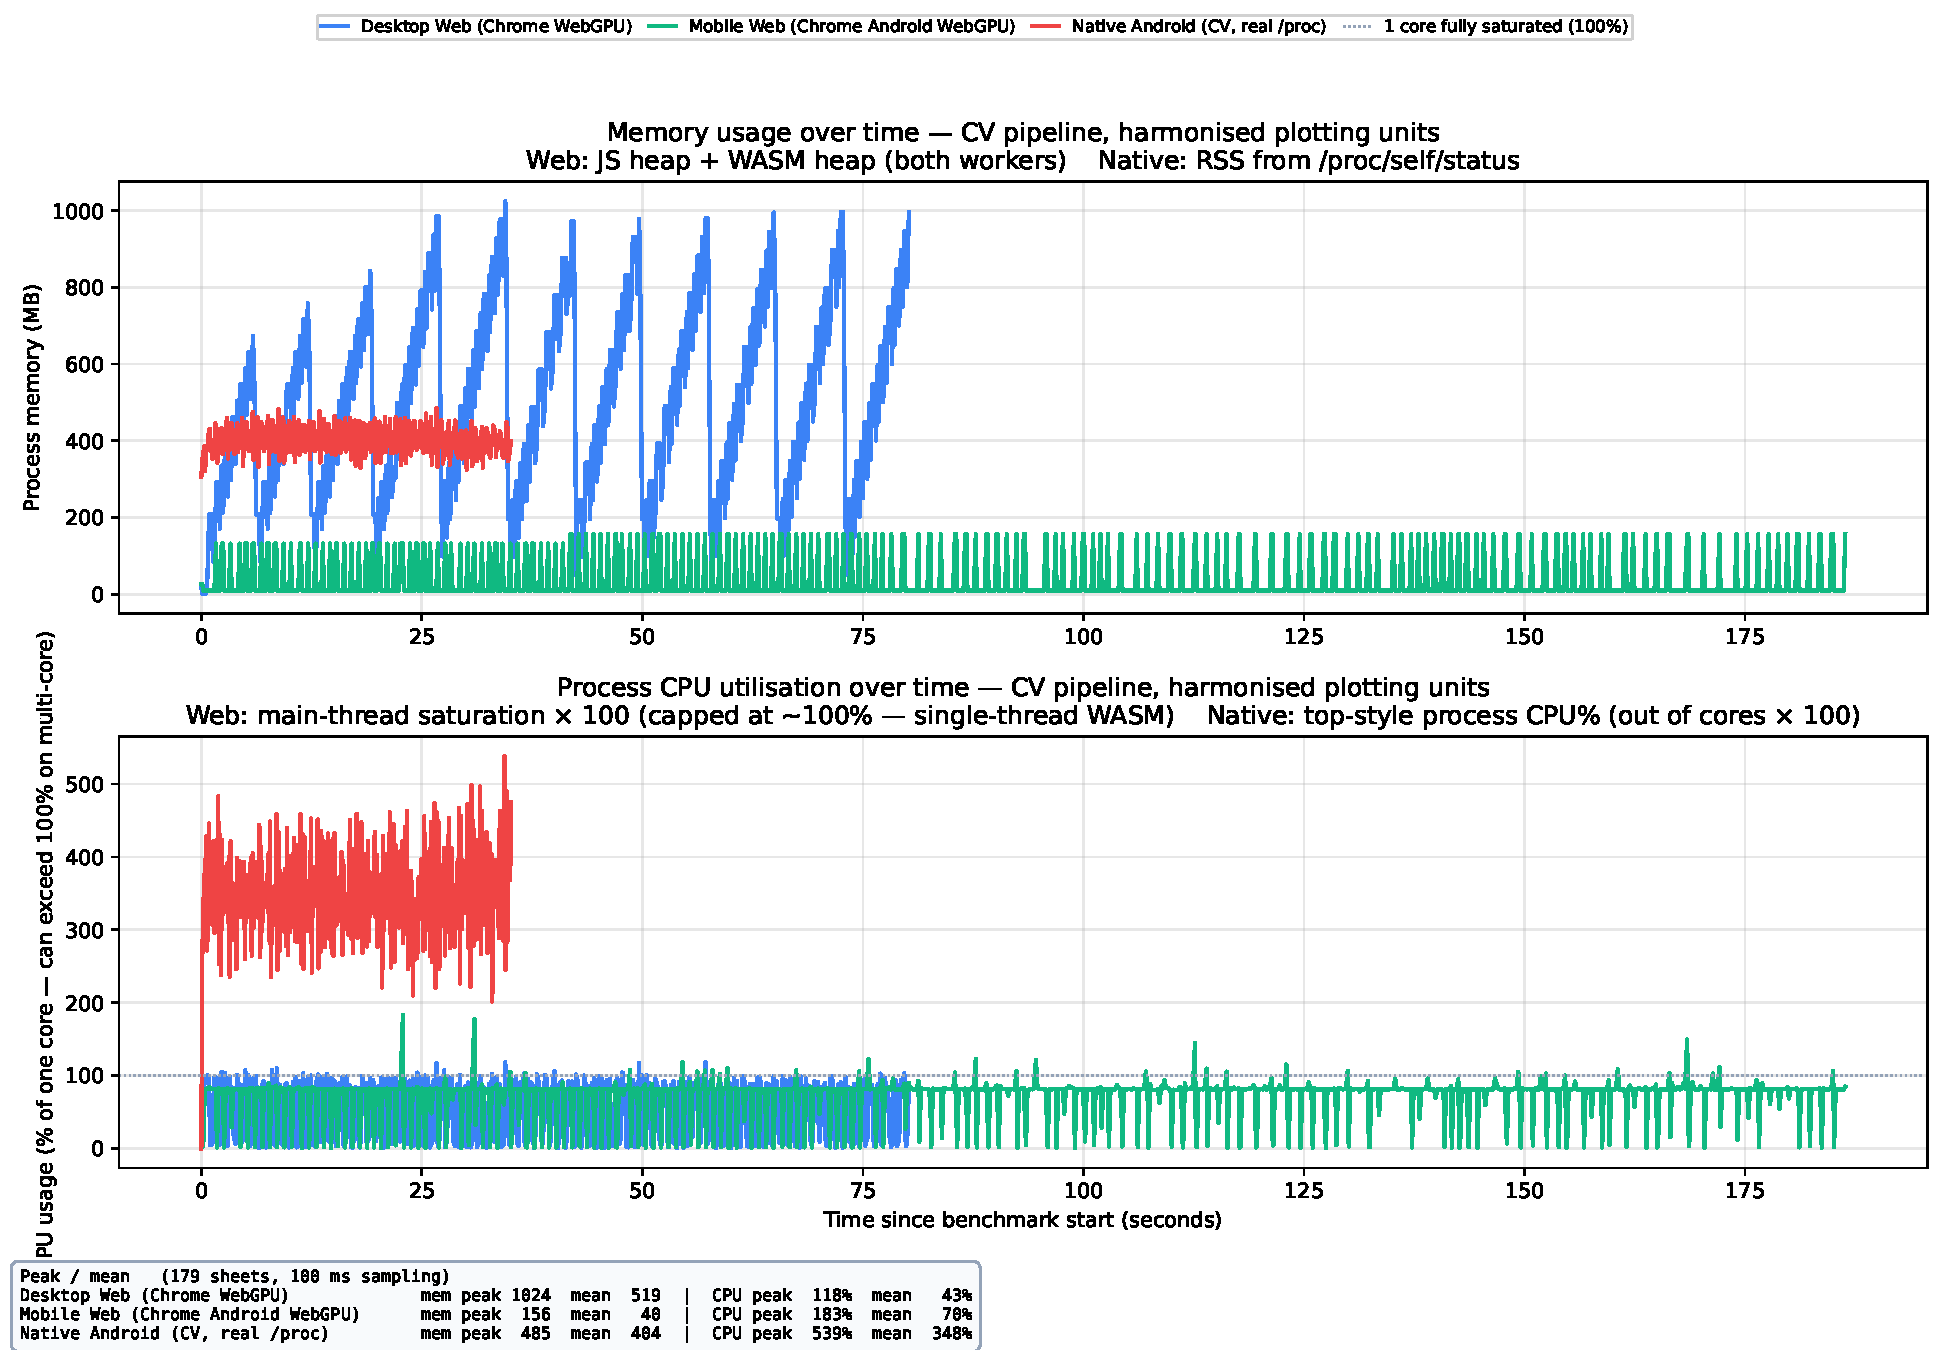
\includegraphics[width=\columnwidth]{figures/chart_cross_platform.pdf}
  \caption{Combined memory and CPU traces for the Traditional CV
  pipeline. Web memory stabilizes early, while Native CPU uses multiple
  cores in bursts.}
  \label{fig:cross_platform}
\end{figure}

The resource traces also explain why lower browser CPU readings should
not be mistaken for higher throughput. The Web worker often remains near
a narrow single-core execution envelope because the deterministic CV
core is compiled into \wasm{} and serialized through its memory model.
Native OpenCV uses more sampled CPU, but converts those bursts into
lower latency through native threading and direct memory access. Resource
boundedness therefore supports deployability, while latency
competitiveness still depends on reducing the \wasm{} CV cost.

\subsection{Threats to Validity}
\label{sec:threats}
\begin{enumerate}[label=(\roman*), leftmargin=*, itemsep=1pt, topsep=2pt]
  \item CPU/RAM instruments differ across platforms, so resource values
  are reported with their native units and used for trend interpretation
  rather than direct cross-instrument ratios.
  \item The supervised accuracy artifact covers one 179-sheet
  fixed-template collection. This is the intended workload scope rather
  than a claim about arbitrary-layout OMR; writer-disjoint data and
  broader capture conditions remain future validation.
  \item Native Android is a latency/resource baseline only. Web and
  Native use matched source-level algorithmic stages, but OpenCV build,
  floating-point ordering, memory layout, and crop-pipeline differences
  can change recognition outputs; Native per-question YOLO labels are
  not exported in the current benchmark.
  \item The YOLO detector is trained on only 56 sheets with an
  11-image validation split (held-out $\mathrm{mAP}@0.5\approx 0.99$).
  The hard-mask ablation shows that a localized bbox can still degrade
  recognition, so bbox-guided cropping should be treated as a separate
  algorithm until validated.
  \item Web latency on thermally constrained laptops is sensitive to the
  host power plan and thermal state. On the Vivobook (i5-13500H) we
  observed up to a $\approx 2\times$ spread in per-sheet \texttt{cpp\_ms}
  across repeated High-Performance runs, driven by CPU/GPU clock
  throttling rather than algorithmic change (recognition outputs are
  bit-identical across runs). The Vivobook row is therefore reported as a
  five-run mean$\pm$std, and the headline Web-vs-Native comparison uses
  the same Redmi device, whose figures reproduced within $\pm5\%$, to
  avoid this confound.
\end{enumerate}

\section{Conclusion}

This benchmark shows that Web Edge OMR is accurate and deployable, but
its latency is governed by stage balance rather than inference alone.
The reviewed Web CV path reaches 99.00\% question accuracy, and YOLO raw
handoff preserves that score, but hard-mask crops fall to 63.70\% and
74.40\%. WebGPU makes YOLO secondary; the remaining gap is dominated by
\wasm{} OMR ($1{,}124$\,ms in the stage profile versus $\approx 88$\,ms
native). If that stage matched native speed, Web YOLO E2E would be
$\approx 387$\,ms, or $1.46\times$ Native NNAPI. Native Android therefore
remains the lower-latency deployment, while Web Edge is the
privacy-preserving, installation-free option whose competitiveness
depends on browser-accessible CV acceleration and \wasm{} runtime
efficiency.

\begin{thebibliography}{11}

\bibitem{patel2015}
R.~Patel, S.~Sanghavi, D.~Gupta, and M.~S.~Raval,
``CheckIt: A low cost mobile OMR system,''
in \textit{Proc. IEEE TENCON}, 2015, pp.~1--6.

\bibitem{okorie2022}
U.~K.~Okorie, O.~Ezenwoye, and T.~H.~Kim,
``Robust image processing based real-time OMR system,''
in \textit{Proc. IEEE CSNT}, 2022, pp.~1--6.

\bibitem{afifi2019}
M.~Afifi and K.~F.~Hussain,
``The achievement of higher flexibility in multiple-choice-based tests
using image classification,''
\textit{IJDAR}, vol.~22, no.~2, pp.~91--126, 2019.

\bibitem{redmon2016}
J.~Redmon, S.~Divvala, R.~Girshick, and A.~Farhadi,
``You Only Look Once: Unified, real-time object detection,''
in \textit{Proc. IEEE CVPR}, 2016, pp.~779--788.

\bibitem{jocher2023}
G.~Jocher, A.~Chaurasia, and J.~Qiu,
``Ultralytics YOLOv8,'' 2023.
[Online]. Available: \url{https://github.com/ultralytics/ultralytics}

\bibitem{tabassum2024}
N.~Tabassum and M.~M.~Rahman,
``An efficient YOLOv8-based OMR system for automated answer sheet
grading,'' in \textit{Proc. ICCCI}, 2024, pp.~1--6.

\bibitem{ali2025}
M.~Ali, S.~Hammoud, and A.~Esper,
``Optical mark recognition techniques for multiple-choice tests:
A comprehensive review,''
\textit{IEEE Access}, vol.~13, pp.~156407--156423, 2025,
doi: 10.1109/ACCESS.2025.3600106.

\bibitem{microsoft2021}
Microsoft,
``ONNX Runtime Web,'' Sep.~2021.
[Online]. Available:
\url{https://opensource.microsoft.com/blog/2021/09/02/onnx-runtime-web-running-your-machine-learning-model-in-browser/}

\bibitem{jangda2019}
A.~Jangda, B.~Powers, E.~Berger, and A.~Guha,
``Not so fast: Analyzing the performance of WebAssembly vs.\ native
code,'' in \textit{Proc. USENIX ATC}, 2019, pp.~107--120.

\bibitem{wang2024}
Q.~Wang \textit{et al.},
``Anatomizing deep learning inference in web browsers,''
\textit{ACM Trans. Softw. Eng. Methodol.}, vol.~34, no.~2, Aug.~2024.

\bibitem{webnn2024}
W3C Machine Learning Working Group,
``Web Neural Network API,'' W3C Candidate Recommendation Draft,
21~May~2026.
[Online]. Available: \url{https://www.w3.org/TR/webnn/}

\end{thebibliography}

\end{document}
